\documentclass[12pt,french]{article}
\input preambule_2013

\newcounter{exoc}
\newenvironment{exoc}[1]{%
  \refstepcounter{exoc}\textbf{Exercice \theexoc} :\hfill {\footnotesize\textbf{(#1)}}\par
  \medskip}%
{\medskip}

\pagestyle{fancy}
\pieddepage{}{\thepage}{}

\setlength{\textheight}{26cm}% Hauteur de la zone de texte

\begin{document}

\begin{center}
\begin{tabularx}{\textwidth}{|>\centering m{2.5cm}|>\centering X|>{\centering\arraybackslash} m{2.5cm}|}
	\hline
		1\iere \bsc{S.t.i.2d.} &  Lundi 7 avril \np{2014} & \textbf{Bilan annuel} \\
	\hline
		\multicolumn{3}{|c|}{\bsc{Correction}} \\
	\hline
\end{tabularx}
\end{center}\bigskip

\begin{exoc}{10 points -- Métropole - La Réunion - 11 septembre 2012}
    \begin{enumerate}
        \item Il y a $32$ femmes sur un total de $48$ personnes donc :
        $p(F) = \dfrac{32}{48} = \dfrac 23.$
        \item Pour calculer $p(E)$, il faut déterminer le nombre de personnes inscrites dans chaque niveau de difficulté :
        \begin{itemize}
        	\item Débutants : $5$ femmes et $2$ hommes donc $7$ randonneurs.
        	\item Moyens : $25 \%$ de $48$ donne $\dfrac{25}{100} \times 48 = 12$ randonneurs ($6$ femmes et $6$ hommes).
        	\item Experts : $48 - 7 - 12 = 29$ randonneurs.
        \end{itemize}
        Finalement : $p(E) = \dfrac{29}{48}$.

        \item $H \cap E$ est l'événement << La randonneur choisi est un homme \textbf{et} il a choisi le niveau élevé >>.\par On sait que $2$ hommes ont choisi le niveau débutant et $6$ hommes ont choisi le niveau moyen donc $8$ hommes ont choisi le niveau élevé donc : $p(H \cap E) = \dfrac{8}{48} = \dfrac 16$.

        \item << Le randonneur est une femme \textbf{ou} choisit l'itinéraire débutant >> se note $F \cup D$.\par On utilise la formule qui est rappelée : $p(F) + p(D) = p(F \cup D) + p(F \cap D)$. On sait que $p(F) =\dfrac{32}{48}$ car il y a $32$ femmes, $p(D) = \dfrac{7}{48}$ car $7$ randonneurs ont choisi le niveau débutant et puisque $5$ femmes ont choisi le niveau débutant $p(F \cap D) = \dfrac{5}{48}$ . Au final :
        \[p(F \cup D) = p(F) + p(D) - p(F \cap D) = \dfrac{32 + 7 - 5}{48} = \dfrac{34}{48} = \dfrac{17}{24}.\]

        \item Dans cette question, on choisit au hasard un randonneur parmi les hommes. L'effectif total est donc ici de $16$ hommes. Puisque $2$ hommes ont choisi le niveau débutant et que $6$ hommes ont choisi le niveau moyen, alors $8$ hommes ont choisi le niveau élevé. Donc, la probabilité que le randonneur ait choisi le niveau élevé \textbf{sachant que c'est un homme} est égal à $\dfrac{8}{16} = \dfrac 1 2$.

        \item $21$ femmes ont choisi le niveau élevé, soit environ $65,6\%$ des femmes ($21 \div 32 = \np{0,65625}$).\par
        D'après la question précédente, $50\%$ des hommes ont choisi le niveau élevé.\par
        On en déduit que le niveau des femmes de ce groupe est plus élevé.
    \end{enumerate}
\end{exoc}\[*\]

\begin{exoc}{8 + 7 = 15 points -- Métropole - La Réunion - 11 septembre 2012 + Antilles - Guyane - 20 juin 2012}

%----------------------------------------------------------------------------
\textbf{Partie} \rond{A}\medskip
%-----------------------------------------------------------------------------

    \begin{enumerate}
        \item $x² = f(x)$ donc $(x - 1)² = f(x - 1)$. Ainsi, $g(x) = f(x - 1) - 4$. D'après le cours, $\calig C_g$ est l'image de $\calig C_f$ par la translation de vecteur $\vect\imath - 4\vect\jmath$.

        \item Le sommet de $\calig C_f$ est le point de coordonnées $(0 \pv 0)$. Par translation, le sommet de $\calig C_g$ a donc pour coordonnées $(1 \pv -4)$.

        \item Tableau de variations de $g$ :
        \begin{center}
        	\begin{tikzpicture}[>=latex]
			\tkzTabInit[nocadre,lgt=3]{$x$/0.75,Variations \\ de $g$/1.5}{$-\infty$,$1$,$+\infty$}
			 \tkzTabVar{+/,-/$-4$,+/}
        	\end{tikzpicture}
        \end{center}

        \item Pour déterminer le signe du trinôme $g$, on peut trouver les racines de $g$.\[g(x) = (x - 1)² - 4 = x² - 2x +1 - 4 = x² - 2x -3.\] Le discriminant est $\Delta = b² - 4ac$ avec $a = 1$, $b = -2$ et $c = -3$. On a alors :
        \[\Delta = (-2)² - 4 \times 1 \times (-3) = 4 + 12 = 16.\]
        Puisque $\Delta > 0$ alors $g$ a deux racines :
        \[\begin{array}{crcl@{\quad \text{et}\quad}rcl}
          	&x_1 & = & \dfrac{-b - \sqrt\Delta}{2a} & x_2 & = & \dfrac{-b + \sqrt\Delta}{2a} \\[8pt]
          	\Leftrightarrow &x_1 & = & \dfrac{-(-2) - \sqrt{16}}{2\times 1} & x_2 & = & \dfrac{-(-2) + \sqrt(16)}{2\times 1} \\[8pt]
          	\Leftrightarrow &x_1 & = & \dfrac{2 - 4}{2} & x_2 & = & \dfrac{2 + 4}{2} \\[8pt]
          	\Leftrightarrow &x_1 & = & -1 & x_2 & = & 3
          \end{array}\]
On en déduit alors le tableau de signes de $g$ :
        \begin{center}
        	\begin{tikzpicture}[>=latex]
			\tkzTabInit[nocadre,lgt=3]{$x$/0.75,Signe \\ de $g$/1.5}{$-\infty$,$-1$,$3$,$+\infty$}
			 \tkzTabLine{,+,z,-,z,+}
        	\end{tikzpicture}
        \end{center}

        \item La calculatrice nous permet de compléter le tableau de valeurs :
        \begin{center}
            \begin{tabular}{*{8}{|>{\centering\arraybackslash}m{1cm}}|}
                \hline
                    $x$ & $-3$ & $-2$ & $-1$ & $0$ & $1$ & $2$ & $3$ \\
                \hline
                    $g(x)$ & $12$ & $5$ & $0$ & $-3$ & $-4$ & $-3$ & $0$ \\
                \hline
            \end{tabular}
        \end{center}
        \item On place les points du tableau de valeurs sur le repère et on les relie par une courbe.
        \begin{center}
		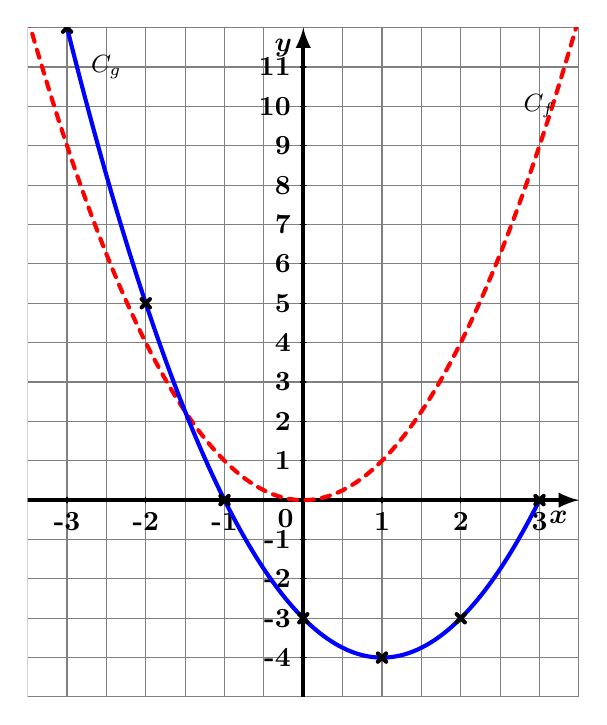
\begin{tikzpicture}[scale=0.5,line cap=round,line join=round, >=latex, x=2cm, y=1cm]
			\clip (-3.5,-5) rectangle (3.5,12);
			\draw[gray] (-3.5,-5)grid(3.5,12);
			\draw[->,line width=1.5pt] (-3.5,0)--(3.5,0)node[below left,font=\boldmath] {$x$};
			\draw[->,line width=1.5pt] (0,-5)--(0,12)node[below left,font=\boldmath] {$y$};
			\foreach \times in {-3,...,-1}
			\draw (\times,2pt) -- (\times,-2pt) node[below,font=\bfseries] {\times};
			\foreach \times in {1,...,3}
			\draw (\times,2pt) -- (\times,-2pt) node[below,font=\bfseries] {\times};
			\foreach \y in {1,...,11}
			\draw[color=black] (2pt,\y) -- (-2pt,\y) node[left,font=\bfseries] {\y};
			\foreach \y in {-4,...,-1}
			\draw[color=black] (2pt,\y) -- (-2pt,\y) node[left,font=\bfseries] {\y};
			\draw (0,0) node [below left,font=\bfseries] {0};
			\draw [smooth,samples=200,domain=-3.5:3.5,line width=1.5pt,color=red,dashed] plot(\x,{(\x)^2}); \draw (3,10) node {\small $\calig C_f$};
			\draw [smooth,samples=200,domain=-3:3,line width=1.5pt,color=blue] plot(\x,{(\x - 1)^2-4}); \draw (-2.5,11) node {\small $\calig C_g$};
			\foreach \x in {-3,...,3}
			\draw [line width=1.5pt] (\x,{(\x - 1)^2-4})-- ++(3pt,3pt)-- ++(-6pt,-6pt)-- ++(3pt,3pt)-- ++(-3pt,3pt)-- ++(6pt,-6pt);
		\end{tikzpicture}
	\end{center}
    \end{enumerate}\medskip

%----------------------------------------------------------------------------
\textbf{Partie} \rond{B}\medskip
%----------------------------------------------------------------------------

\begin{enumerate}
    \item $t(0) = a \times 0² + b\times 0 + c = c$ donc le cœfficient $c$ est l'image de $0$. Graphiquement, on lit $c = 3$.

    \item D'après l'énoncé, le point $S\left(\dfrac 12\pv 4\right)$ est le sommet de la parabole $\calig P$.\par
    L'abscisse du sommet d'une parabole est égale à $\dfrac{-b}{2a}$ donc :
    \[\dfrac{-b}{2a} = \dfrac 12 \qLRq -b = \dfrac 12 \times 2a \qLRq -b = a \qLRq a + b = 0.\]

    \item $t(\frac 12) = 4$ donc $a \times (\frac 1 2)² + b \times \frac 12 + 3 = 4$.
    \[\frac{a}{4} + \frac{b}{2} = 4 - 3 \qLRq \frac{a + 2b}{4} = 1 \qLRq a + 2b = 4.\]

    \item
    \[
    	\left\{
		\begin{array}{rcl}
			a + b & = & 0 \\
			a + 2b & = & 4
		\end{array}
    	\right. \qLRq
	\left\{
		\begin{array}{rcl}
			a & = & -b \\
			-b + 2b & = & 4
		\end{array}
    	\right. \qLRq
    	\left\{
		\begin{array}{rcl}
			a & = & -4 \\
			b & = & 4
		\end{array}
    	\right.
    \]
Ainsi, $t(x) = -4x² + 4x + 3$.

    \item Le discriminant de $t$ est $\Delta = b² - 4ac$ avec $a = -4$, $b = 4$ et $c = 3$. On a alors :
        \[\Delta = 4² - 4 \times (-4) \times 3 = 16 + 48 = 64.\]
        Puisque $\Delta > 0$ alors $t$ a deux racines :
        \[\begin{array}{crcl@{\quad \text{et}\quad}rcl}
          	&x_1 & = & \dfrac{-b - \sqrt\Delta}{2a} & x_2 & = & \dfrac{-b + \sqrt\Delta}{2a} \\[8pt]
          	\Leftrightarrow &x_1 & = & \dfrac{-4 - \sqrt{64}}{2\times (-4)} & x_2 & = & \dfrac{-4 + \sqrt(64)}{2\times (-4)} \\[8pt]
          	\Leftrightarrow &x_1 & = & \dfrac{-4 - 8}{-8} & x_2 & = & \dfrac{-4 + 8}{-8} \\[8pt]
          	\Leftrightarrow &x_1 & = & \dfrac{-12}{-8} = \dfrac 32 & x_2 & = & \dfrac{4}{-8} = \dfrac{-1}{2}
          \end{array}\]
\end{enumerate}
\end{exoc}\[*\]

\begin{exoc}{7 + 8 = 15 points -- Antilles - Guyane - 19 juin 2013}

%----------------------------------------------------------------------------
\textbf{Partie} \rond{A}\medskip
%-----------------------------------------------------------------------------

\begin{enumerate}
	\item La solution de l'équation $(2-\ii)z = 2 - 6\ii$ est le nombre $z_1$ tel que :
	\[z_1 = \dfrac{2 - 6\ii}{2-\ii} = \dfrac{(2-6\ii)(2+\ii)}{(2-\ii)(2+\ii)} = \dfrac{10 - 10\ii}{5} = 2 - 2\ii.\]
	
	\item On calcule tout d'abord le module de $z_1$ :
	\[\abs{z_1} = \abs{2 - 2\ii} = \sqrt{2² + (-2)²} = \sqrt{4 + 4} = \sqrt 8 = 2\sqrt 2.\]
	Puis on factorise par $\abs{z_1}$ pour obtenir :
	\[z_1 = 2\sqrt2\left(\dfrac{2}{2\sqrt2} - \dfrac{2}{2\sqrt2}\ii\right)
		   = 2\sqrt2\left(\dfrac{1}{\sqrt2} - \dfrac{1}{\sqrt2}\ii\right)
		   = 2\sqrt2\left(\dfrac{\sqrt 2}{2} - \dfrac{\sqrt 2}{2}\ii\right)\]
	En notant $\theta = \arg(z_1)$, on en déduit que :
	\[\left.\begin{array}{rcl}
	  	\cos(\theta)& = &\frac{\sqrt2}{2}\\[5pt]
	  	\sin(\theta) & = & -\frac{\sqrt2}{2}
	  \end{array}\right\} \qRq \theta = -\dfrac\pi4\]
	  Ainsi, $z_1 = \left[2\sqrt 2 \pv -\dfrac\pi 4\right]$.

	\item $z_2 = -\ii\times z_1 = -\ii (2 - 2\ii) = -2\ii + 2 \ii² = -2 - 2\ii$.
	
	Pour la forme trigonométrique, on réalise les mêmes calculs que pour $z_1$ en faisant attention aux signes et on trouve $\abs{z_2} = 2\sqrt 2$ et :
	\[\left.\begin{array}{rcl}
		\cos(\theta)& = &-\frac{\sqrt2}{2}\\[5pt]
		\sin(\theta) & = & -\frac{\sqrt2}{2}
	  \end{array}\right\} \qRq \theta = -\dfrac{3\pi}{4}\]
	  Ainsi, $z_2 = \left[2\sqrt 2 \pv -\dfrac{3\pi}{4}\right]$.
\end{enumerate}\medskip

%----------------------------------------------------------------------------
\textbf{Partie} \rond{B}\medskip
%-----------------------------------------------------------------------------

            \begin{enumerate}
                \item On doit faire attention à l'unité définie par les vecteurs $\vect u$ et $\vect v$.
			\begin{center}
			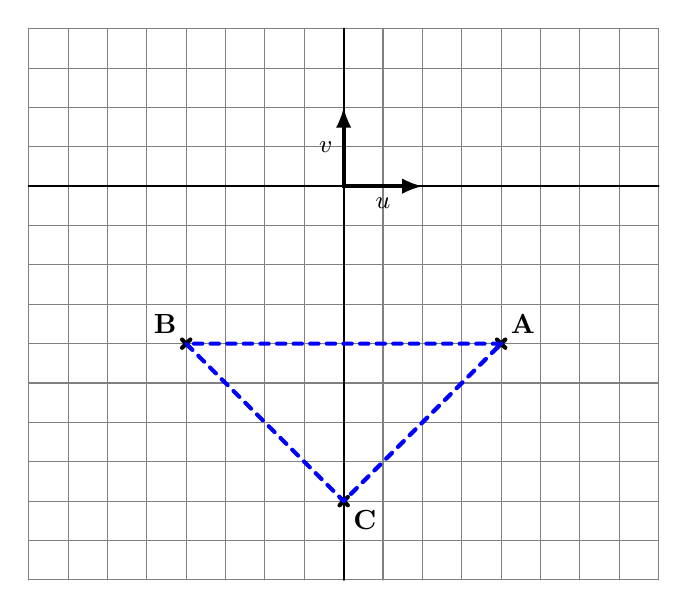
\begin{tikzpicture}[scale=0.5, line cap=round, line join=round, >=latex, x=2cm, y=2cm]
				\draw[gray] (-4,-5)grid(4,2);
				\draw[-,line width=0.75pt] (-4,0)--(4,0);
				\draw[-,line width=0.75pt] (0,-5)--(0,2);
				\draw[->, line width = 1.5pt] (0,0) -- (1,0) node[below,midway] {\small $\vect u$};
				\draw[->, line width = 1.5pt] (0,0) -- (0,1) node[left,midway] {\small $\vect v$};
				\coordinate (A) at (2,-2);
				\draw (A) node [above right,font=\bfseries] {A};
				\draw [line width=1.5pt] (A)-- ++(3pt,3pt)-- ++(-6pt,-6pt)-- ++(3pt,3pt)-- ++(-3pt,3pt)-- ++(6pt,-6pt);
				\coordinate (B) at (-2,-2);
				\draw (B) node [above left,font=\bfseries] {B};
				\draw [line width=1.5pt] (B)-- ++(3pt,3pt)-- ++(-6pt,-6pt)-- ++(3pt,3pt)-- ++(-3pt,3pt)-- ++(6pt,-6pt);
				\coordinate (C) at (0,-4);
				\draw (C) node [below right,font=\bfseries] {C};
				\draw [line width=1.5pt] (C)-- ++(3pt,3pt)-- ++(-6pt,-6pt)-- ++(3pt,3pt)-- ++(-3pt,3pt)-- ++(6pt,-6pt);
				\draw[line width = 1.5pt, color=blue,dashed] (A) -- (B)-- (C)-- cycle;
			\end{tikzpicture}
			\end{center}
			
                \item
			$z_3 = z_{\vect{CA}}= z_A - z_C = 2 - 2\ii - (-4\ii) = 2 + 2\ii$.\par
			$z_4 = z_{\vect{CB}} = z_B - z_C = -2 - 2\ii - (-4\ii) = -2 + 2\ii$.
			
                \item Les affixes des vecteurs nous permettent de connaître leurs coordonnées donc :\[\vect{CA}\binom{2}{2} \qetq \vect{CB}\binom{-2}{2}.\] Donc : $\vect{CA}\cdot \vect{CB} = xx' + yy' = 2 \times (-2) + 2 \times 2 = -4 + 4 = 0$. On en déduit que les vecteurs $\vect{CA}$ et $\vect{CB}$ sont orthogonaux donc $(CA) \perp (CB)$.

                \item
			$\norme{\vect{CA}} = \abs{z_3} = 2\sqrt 2$ et $\norme{\vect{CB}} = \abs{z_4} = 2\sqrt 2$. On en déduit que les longueurs $AC$ et $CB$ sont égales.
			
                \item D'après les deux questions précédentes, on en déduit que le triangle $ABC$ est \textbf{rectangle et isocèle en $C$}.
            \end{enumerate}
\end{exoc}

\end{document} 